%6/27 tb ⇒ t
\begin{figure}[t]
    \centering
    \subfloat[Normals]{
      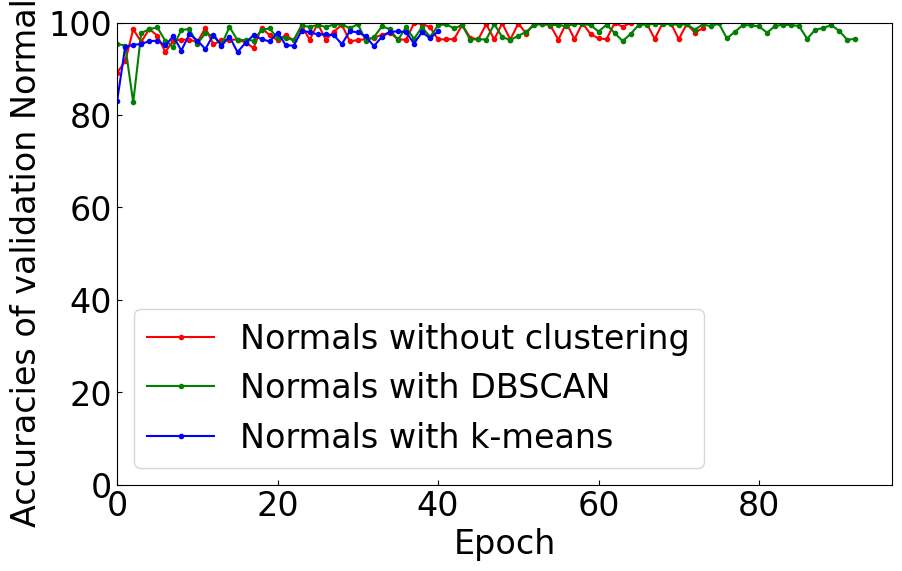
\includegraphics[width=.45\linewidth]{img/Accuracies_of_validation_normals.png}
      \label{valnormal}
    }
    \subfloat[Dimensionality features]{
      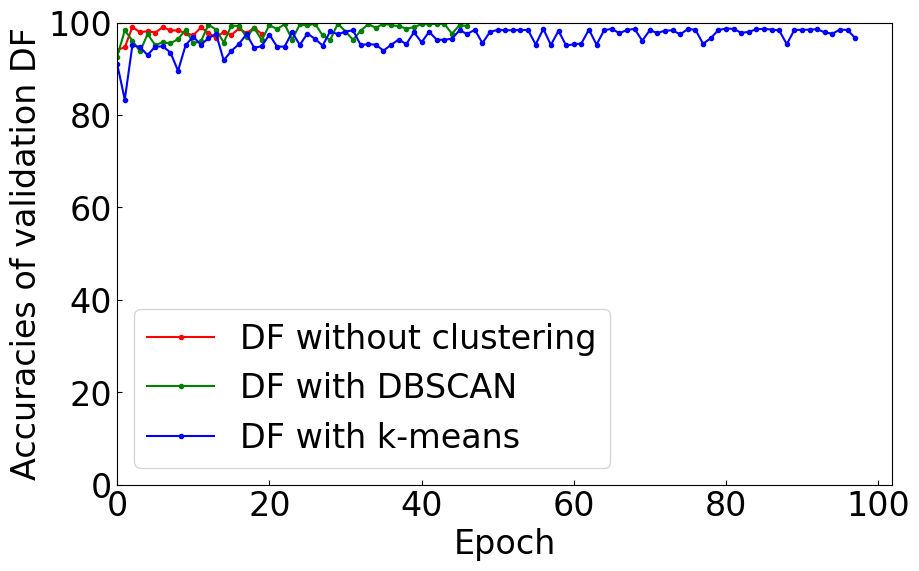
\includegraphics[width=.45\linewidth]{img/Accuracies_of_validation_DF.png}
      \label{valdim}
    }
    \\
    \subfloat[Proportion of variances]{
      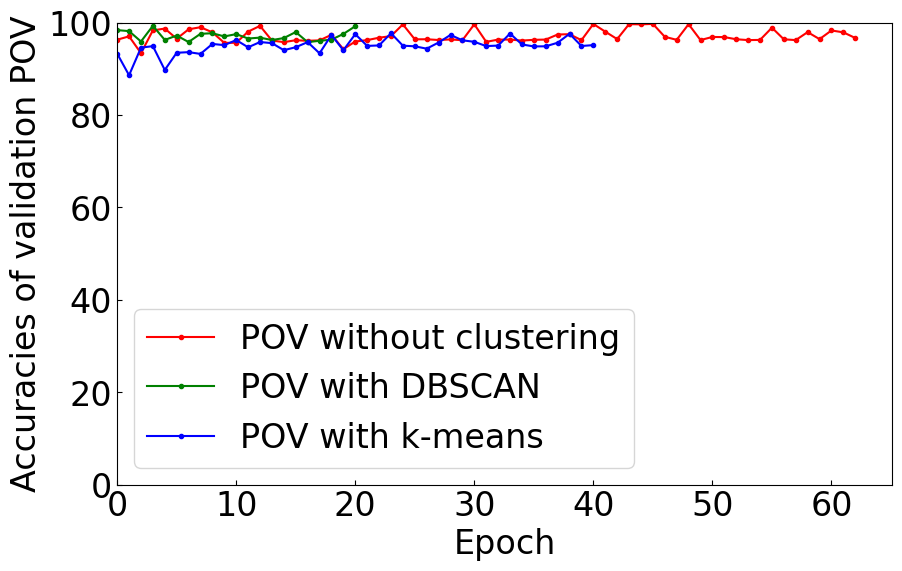
\includegraphics[width=.45\linewidth]{img/Accuracies_of_validation_POV.png}
      \label{valproportion}
    }
    \subfloat[FPFH]{
      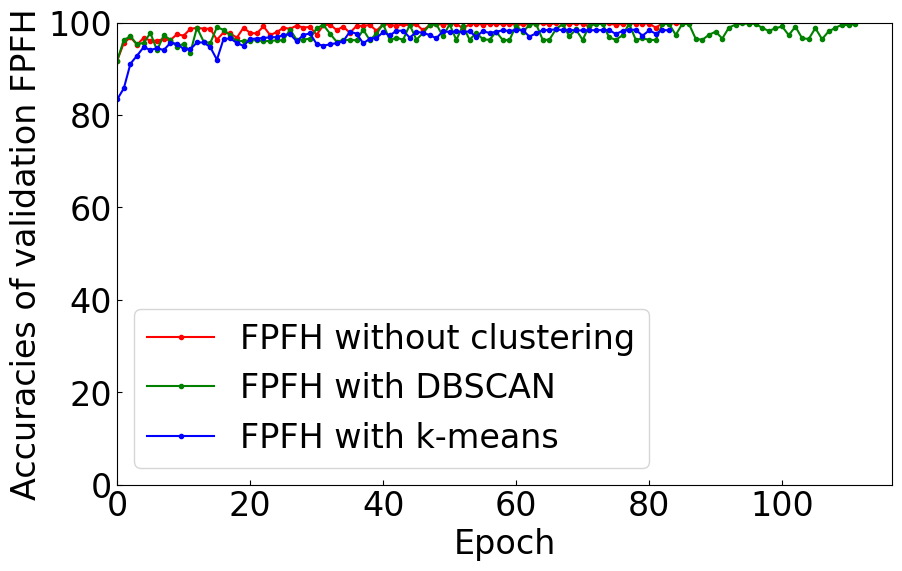
\includegraphics[width=.45\linewidth]{img/Accuracies_of_validation_FPFH.png}
      \label{valfpfh}
    }
    \caption{Classification accuracies of validation.}
    \label{valacc}
  \end{figure} 

%1st paragraph
%1概要
\deleted{Fig.~\ref{valacc} show graphs of the validation per epoch when using each feature.}
\deleted{%2各表の折れ線グラフの説明
Each figure has three line graphs, each with no clustering, with DBSCAN, and with k-means.}
\revised{Fig.~\ref{valacc} plots validation accuracy per epoch for each feature with no clustering, DBSCAN, and k-means.}
\begin{deletedblock}
%2nd paragraph
%1法線を使った分類モデル
Fig.~\ref{valacc}\subref{valnormal} shows the accuracies of three types classification models when the normals were used. 
    %1-1
    As shown, the overall accuracies are nearly 100\%. 
%2The dimensionality featuresを使った分類モデル
Fig.~\ref{valacc}\subref{valdim} shows the accuracies of three types classification models when the dimensionality features were used. 
    %2-1
    As shown, the overall accuracies are nearly 100\%. 
%3The proportion of varianceを使った分類モデル
Fig.~\ref{valacc}\subref{valproportion} shows the accuracies of three types classification models when the proportion of variance was used. 
  %3-1
  As shown, the overall accuracies are nearly 100\%. 
%4FPFHの分類モデル
Fig.~\ref{valacc}\subref{valfpfh} shows the accuracies of three types classification models when the FPFH was used. 
  %4-1
  As shown, the overall accuracies are nearly 100\%. 
\end{deletedblock}
%2
\revised{All four features achieved nearly 100\% validation accuracy across clustering methods.}

%2nd paragraph
%5エポック数の決定
\deleted{The training epochs for each classification model were set so that after updating the best accuracy in validation, training would be terminated if there were no updates within 15 epochs.}
\revised{Training was terminated after 15 epochs without validation-accuracy improvement beyond the best value.}
